% !TeX program = xelatex
% ============================================================
%  《系统开发工具基础》实验报告 —— 第 1 周
%  姓名：徐宜安  学号：25060012033
%  编译：latexmk -pdf -halt-on-error 实验报告.tex（.latexmkrc 已固定 XeLaTeX）
% ============================================================
\documentclass[12pt,a4paper,fontset=fandol]{ctexart}

% ---------- 页面布局 ----------
\usepackage[a4paper,margin=2.3cm]{geometry}
\setlength{\headheight}{14pt}

% ---------- 数学 ----------
\usepackage{amsmath,amssymb}

% ---------- 图片 ----------
\usepackage{graphicx}
\graphicspath{{课上/q01/}{课上/q02/}{课上/q03/}{课上/q04/}}

% ---------- 表格 ----------
\usepackage{booktabs,array,multirow}

% ---------- 颜色与代码高亮 ----------
\usepackage{xcolor}
\definecolor{codebg}{HTML}{f6f8fa}
\definecolor{codeframe}{HTML}{d0d7de}
\definecolor{kwred}{HTML}{cf222e}
\definecolor{strblue}{HTML}{0a3069}
\definecolor{cmtgray}{HTML}{6e7781}
\definecolor{fnpurple}{HTML}{8250df}
\definecolor{numblue}{HTML}{0550ae}

\usepackage{listings}
\renewcommand{\lstlistingname}{代码}

% shell 风格语言：第一组为常用命令，第二组为 git 子命令
\lstdefinelanguage{shell}{
  morekeywords={mkdir,cd,echo,touch,cp,rm,mv,find,chmod,chown,pwd,ls,cat,head,tail,sort,uniq,awk,sed,grep,printf,exit,return,if,then,else,elif,fi,do,done,for,in,while,case,esac,trap,sleep,bg,jobs,kill,wait,set,export,source,local,time},
  morekeywords=[2]{git,init,add,commit,checkout,merge,log,status,branch,clone,push,pull,diff,stash,restore,switch},
  morecomment=[l]{\#},
  morestring=[b]",
  morestring=[b]',
  sensitive=true,
}

% 简单的 Python 风格（课后练习示例用）
\lstdefinelanguage{py}{
  morekeywords={import,from,def,return,if,else,elif,for,in,while,print,with,open,as,class,assert,random,seed,range,lambda},
  morecomment=[l]{\#},
  morestring=[b]",
  morestring=[b]',
}

% GitHub 浅色风格代码块
\lstdefinestyle{labcode}{
  backgroundcolor=\color{codebg},
  basicstyle=\small\ttfamily,
  keywordstyle=\color{kwred}\bfseries,
  keywordstyle=[2]\color{fnpurple}\bfseries,
  commentstyle=\color{cmtgray}\itshape,
  stringstyle=\color{strblue},
  numberstyle=\tiny\color{cmtgray},
  numbers=left,
  frame=single,
  rulecolor=\color{codeframe},
  breaklines=true,
  breakatwhitespace=false,
  showstringspaces=false,
  tabsize=4,
  columns=fullflexible,
  keepspaces=true,
  captionpos=b,
  xleftmargin=1.6em,
  framexleftmargin=1.2em,
  aboveskip=0.6em,
  belowskip=0.6em,
}
\lstset{style=labcode}

% ---------- 页眉页脚 ----------
\usepackage{fancyhdr}
\usepackage{lastpage}
\pagestyle{fancy}
\fancyhf{}
\fancyhead[L]{\small 系统开发工具基础 · 实验报告}
\fancyhead[R]{\small 徐宜安\quad 25060012033}
\fancyfoot[C]{\small 第 \thepage\ 页 / 共 \pageref{LastPage} 页}
\renewcommand{\headrulewidth}{0.4pt}

% ---------- 超链接 ----------
\usepackage{hyperref}
\hypersetup{colorlinks=true,linkcolor=numblue,urlcolor=numblue,citecolor=numblue}

% ---------- 题目要求框 ----------
\usepackage{tcolorbox}
\tcbuselibrary{breakable}
\newtcolorbox{taskbox}[1][]{
  colback=blue!4!white,
  colframe=blue!50!black,
  fonttitle=\bfseries,
  title={#1},
  boxrule=0.6pt,
  arc=1.5pt,
  left=8pt, right=8pt, top=5pt, bottom=5pt,
  breakable,
}

% ---------- 图表说明样式 ----------
\usepackage{caption}
\captionsetup{font=small,labelfont=bf,labelsep=quad}

% ---------- 列表 ----------
\usepackage{enumitem}

% ==================== 每周填写区 ====================
\newcommand{\weeknum}{第 1 周}
\newcommand{\weektheme}{课程概览与 Shell 入门 · Version Control and Git · LaTeX 文档编辑}
\newcommand{\classdate}{2026 年 8 月 24 日}
% ==================== 每周填写区结束 ====================

% 首页标题块（姓名/学号等信息在此修改）
\newcommand{\makereporttitle}{%
  \begin{center}
    {\LARGE\bfseries 系统开发工具基础 · 实验报告}\\[0.4em]
    {\normalsize \weeknum：\weektheme}\\[0.7em]
    {\small
    \begin{tabular}{@{}ll@{\hspace{3em}}ll@{}}
      姓\quad 名 & 徐宜安 & 学\quad 号 & 25060012033 \\
      授课教师 & 周小伟 & 上课日期 & \classdate \\
      Git 仓库 & \href{https://github.com/xya-123/Fundamentals-of-Computer-System-Development-Tools}{GitHub 课程仓库} & 报告日期 & \today \\
    \end{tabular}}\\[0.7em]
    \rule{\textwidth}{0.8pt}
  \end{center}
}

\begin{document}
\makereporttitle

\section{课上练习}

% ================= q01 =================
\subsection{q01 · 含空格文件名的批量整理（Shell 基础与文件系统）}

\begin{taskbox}[题目要求]
在当前目录新建 q01 并完全使用命令行完成：
\begin{itemize}[nosep]
  \item 创建 \texttt{input/docs} 与 \texttt{input/tmp}，并创建四个文件：\texttt{notes one.txt}（alpha、beta 两行）、\texttt{.secret.txt}（隐藏文件）、\texttt{empty.txt}（空文件）、\texttt{run.log}（任意两行日志）；
  \item 显示 q01 的绝对路径，以长格式列出 input 下全部项目，包含隐藏文件；
  \item 把 input 下所有 \texttt{.txt} 文件复制到 \texttt{work/<学号>/}，保留相对目录结构并正确处理名称中的空格；
  \item 复制后的目录权限设为 750、普通文件权限设为 640；生成 \texttt{inventory.txt}，列出相对路径和字节数。
\end{itemize}
\end{taskbox}

\textbf{实现思路：} 含空格的文件名必须作为一个完整参数传递；如果不加引号，
Shell 会把 \texttt{notes one.txt} 拆成两个参数。
脚本使用 \texttt{find -exec cp -{}-parents} 逐个复制匹配到的文件，
并用 \texttt{-{}-parents} 保留原目录结构。随后分别对目录和普通文件设置
750、640 权限，再用 \texttt{-printf "\%P \%s"} 生成相对路径与字节数清单。
完整脚本见代码~\ref{lst:q01}，分步执行过程见图~\ref{fig:q01-steps}。

\begin{figure}[htbp]
  \centering
  \resizebox{0.78\textwidth}{!}{%
    \vbox{\offinterlineskip
      \hbox{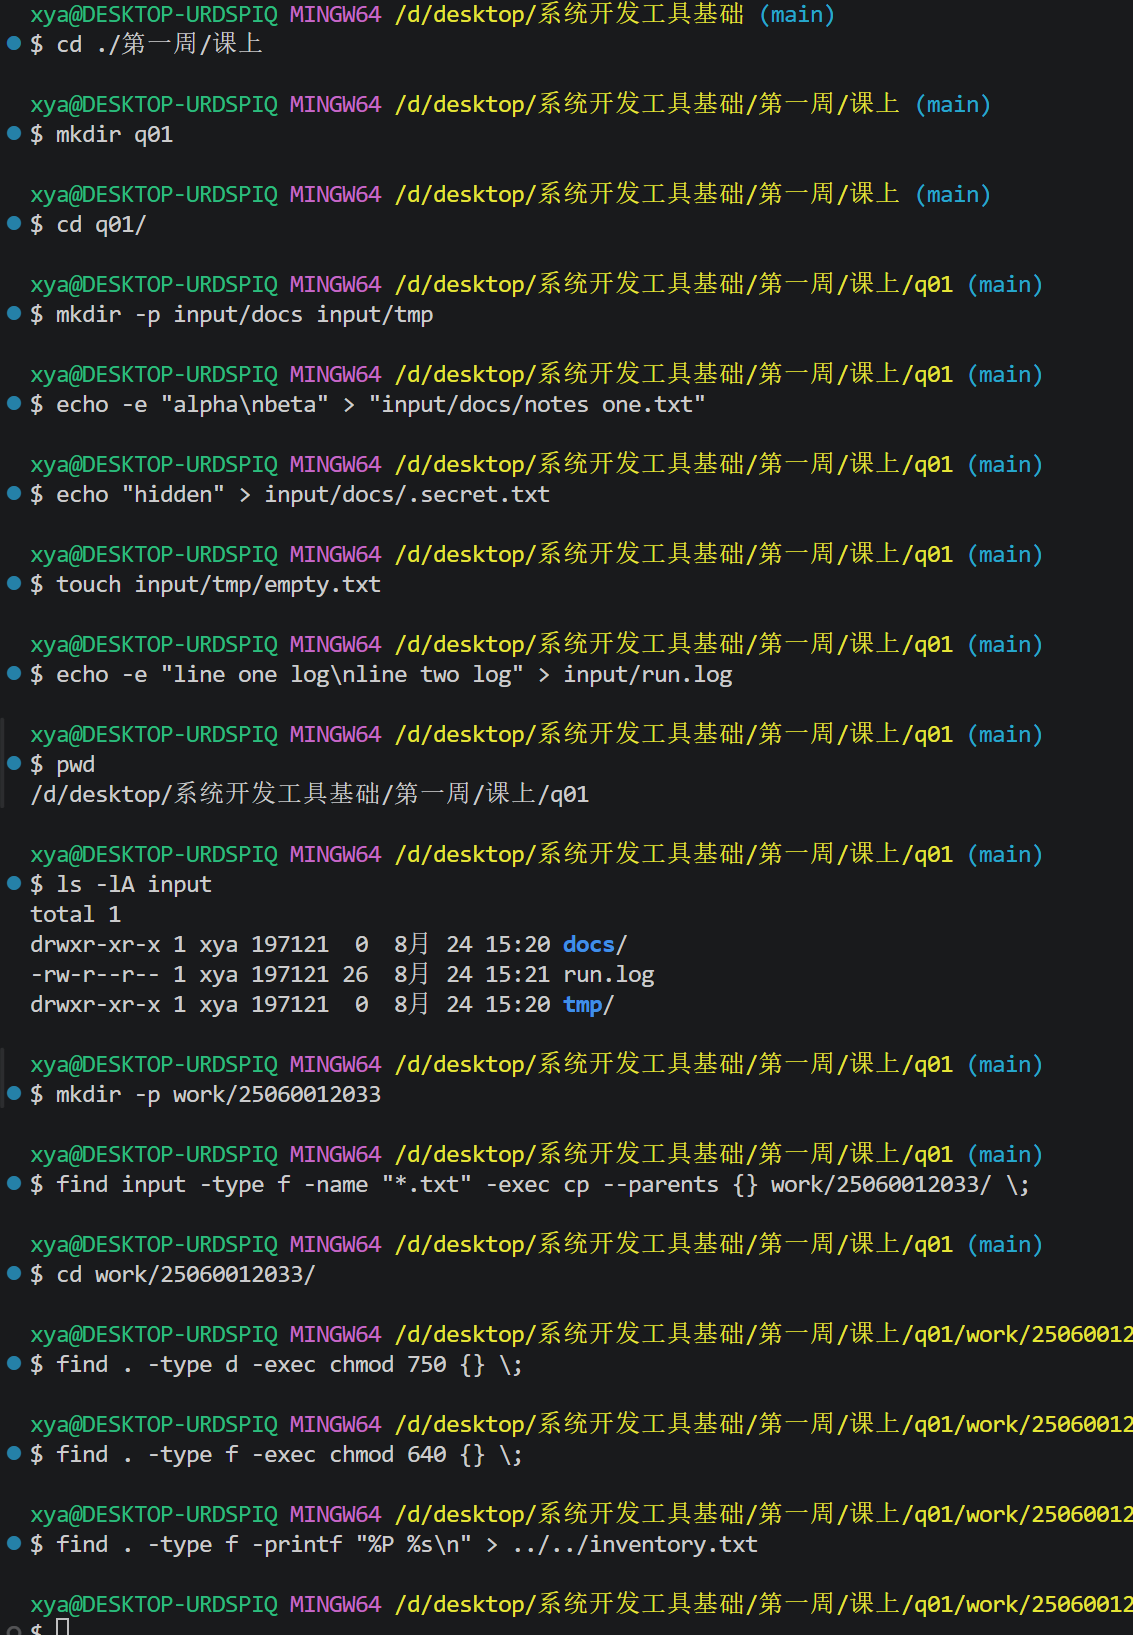
\includegraphics[trim=0 345bp 0 0,clip]{课上/q01/分布命令1.png}}%
      \hbox{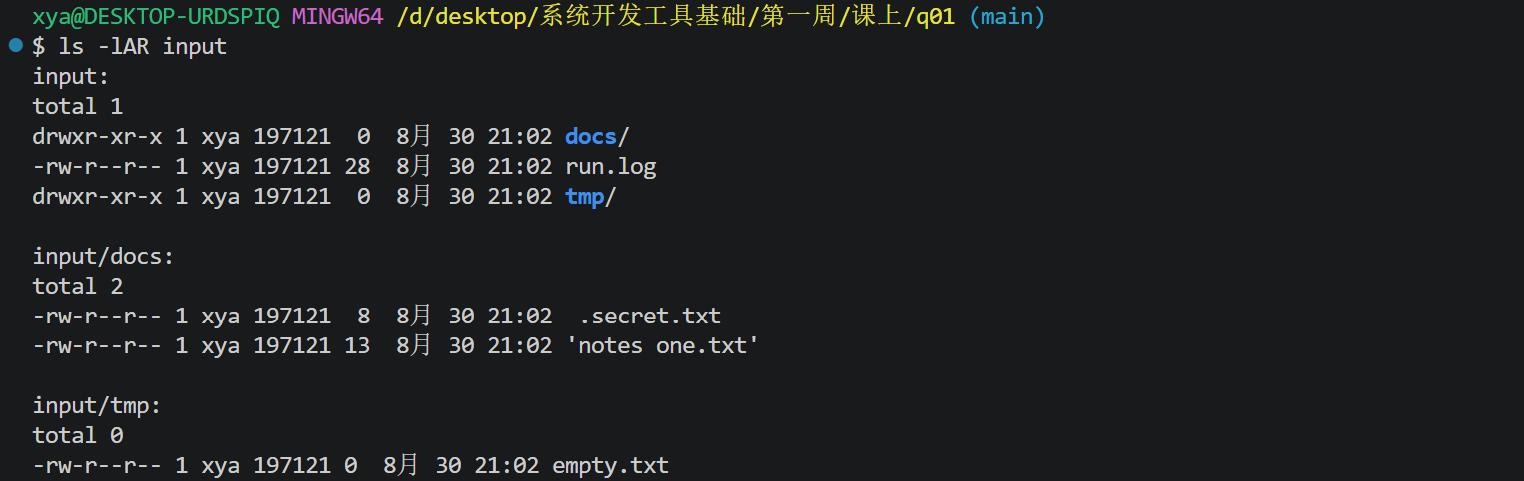
\includegraphics[trim=0 0 167.6bp 0,clip]{课上/q01/分布命令2.png}}%
      \hbox{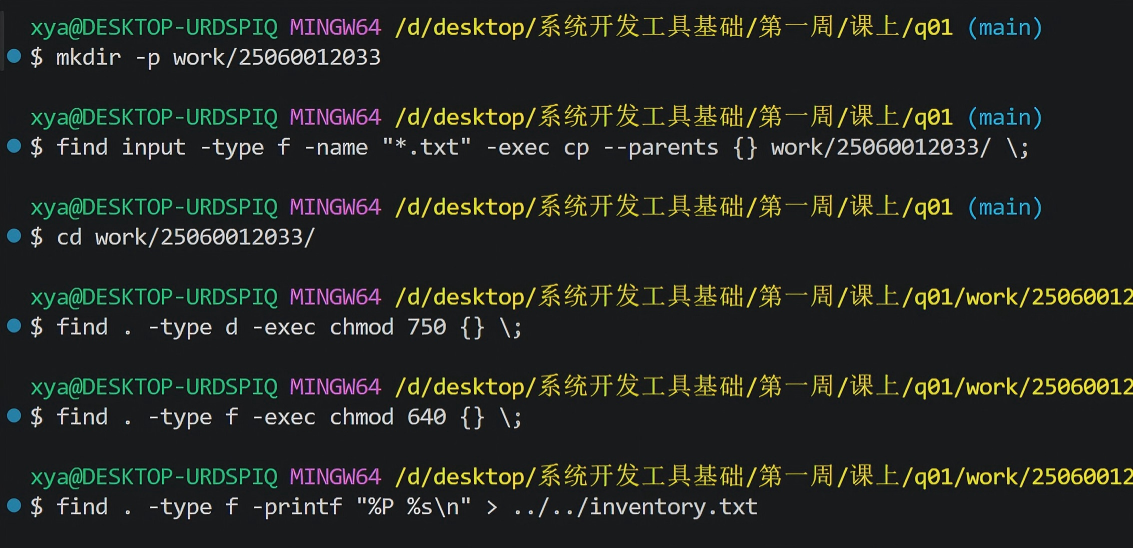
\includegraphics{课上/q01/分步命令3.png}}%
    }%
  }
  \caption{q01 分步命令执行过程（终端截图）}
  \label{fig:q01-steps}
\end{figure}

\lstinputlisting[caption={q01.sh：批量整理总脚本},label={lst:q01}]{课上/q01/q01.sh}

\textbf{结果：} 复制后的目录结构见代码~\ref{lst:q01-tree}。
\texttt{run.log} 因扩展名不符而未复制，三个 \texttt{.txt} 文件均保留了原目录结构。
\texttt{inventory.txt} 的结果见代码~\ref{lst:q01-inv}，三个文件的字节数分别为
7、11 和 0；目录权限设为 750，文件权限设为 640。
图中重新执行 \texttt{ls} 时显示为 8、13 和 0 字节，是因为文件后来使用了 Windows 的
CRLF 换行；清单生成时使用的是 LF 换行，可见文本内容没有变化。

\begin{lstlisting}[language=shell,caption={q01 最终目录结构（work/ 下仅复制 .txt 文件）},label={lst:q01-tree}]
q01/
|-- input/
|   |-- docs/
|   |   |-- .secret.txt         # 隐藏文件
|   |   `-- notes one.txt       # 含空格文件名
|   |-- tmp/
|   |   `-- empty.txt           # 空文件
|   `-- run.log
|-- work/
|   `-- 25060012033/
|       `-- input/              # 仅 .txt 被复制
|           |-- docs/           # .secret.txt, notes one.txt
|           `-- tmp/            # empty.txt
|-- inventory.txt
`-- q01.sh
\end{lstlisting}

\begin{lstlisting}[language=,caption={inventory.txt：复制清单（相对路径 + 字节数）},label={lst:q01-inv}]
input/docs/.secret.txt 7
input/docs/notes one.txt 11
input/tmp/empty.txt 0
\end{lstlisting}

% ================= q02 =================
\subsection{q02 · 随机访问日志统计（Shell 管道与文本处理）}

\begin{taskbox}[题目要求]
在 q02 中创建 access.csv，并完成日志统计：
\begin{itemize}[nosep]
  \item 编写 analyze.sh，接收一个 CSV 文件路径；文件不存在时将错误写入 stderr 并返回非零退出码；
  \item 使用 Shell 管道以及 awk、sort、head 等工具，输出 HTTP 5xx 数量最多的前 2 个 path；按次数降序，次数相同时按 path 字典序；
  \item 输出全部数据行的平均 latency\_ms，保留两位小数；表头不得计入；
  \item 分别对 access.csv 和一个不存在的文件运行脚本；不得使用 Python、电子表格或手工统计。
\end{itemize}
\end{taskbox}

\textbf{实现思路：} 脚本先检查输入文件是否存在，不存在时向 stderr 输出错误并
以状态码 1 退出。统计部分分为三步：
\begin{itemize}[nosep]
  \item 过滤与提取：\texttt{awk -F',' 'NR>1 \&\& \$4 \textasciitilde{} /\textasciicircum{}5/ \{print \$3\}'}——逗号分隔、跳过表头、status 以 5 开头时输出 path；
  \item 计数与排序：\texttt{sort | uniq -c | sort -k1,1nr -k2,2 | head -n 2}——先按次数数值降序、次数相同时按 path 字典序，取前 2；
  \item 平均值：awk 累加 \texttt{\$5}，END 块用 \texttt{printf "\%.2f"} 保留两位小数，表头由 \texttt{NR>1} 排除。
\end{itemize}
完整实现见代码~\ref{lst:q02}。

\lstinputlisting[caption={analyze.sh：访问日志统计脚本},label={lst:q02}]{课上/q02/analyze.sh}

\textbf{结果：} 运行结果见图~\ref{fig:q02-result}。5xx 数量最多的两个 path 是
\texttt{/api/orders}（3 次）和 \texttt{/api/users}（2 次），8 条记录的平均延迟为
193.75 ms。传入不存在的文件时，脚本向 stderr 报错并返回状态码 1。

\begin{figure}[htbp]
  \centering
  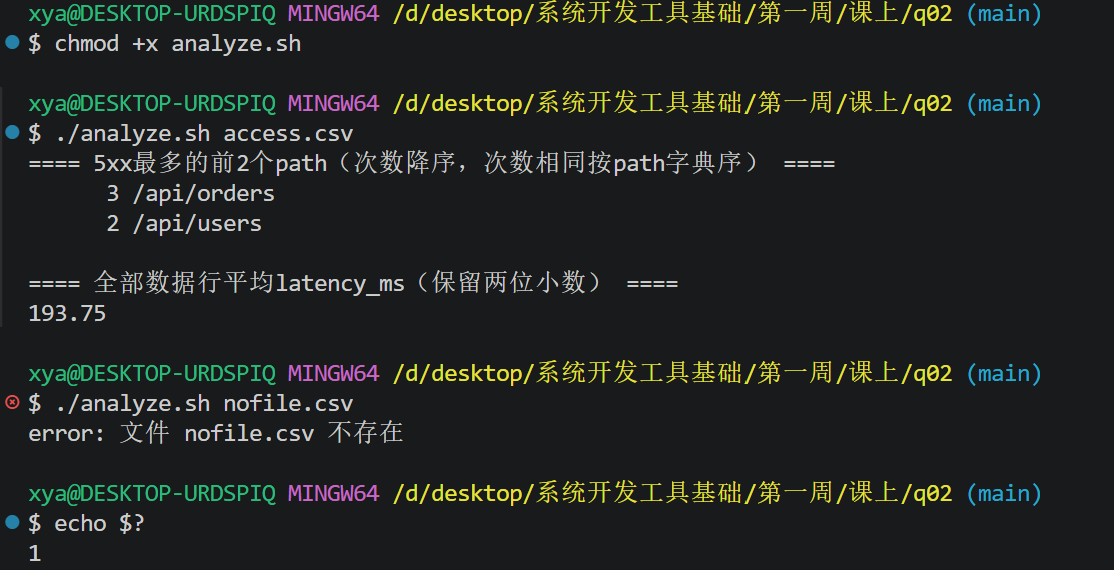
\includegraphics[width=0.85\textwidth]{结果.png}
  \caption{q02 运行结果：5xx 统计、平均延迟与错误分支（终端截图）}
  \label{fig:q02-result}
\end{figure}

% ================= q03 =================
\subsection{q03 · 制造、解决并解释一次合并冲突（Version Control and Git）}

\begin{taskbox}[题目要求]
在 q03 中从零创建一个 Git 仓库，并主动制造、解决一次合并冲突：
\begin{itemize}[nosep]
  \item 初始化仓库，在 main 创建 \texttt{config.txt}（\texttt{mode=normal}）并完成初始提交；
  \item 创建 feature-a 改为 \texttt{mode=safe} 并提交；从初始 main 创建 feature-b 改为 \texttt{mode=fast} 并提交；
  \item 回到 main，先合并 feature-a，再合并 feature-b；解决冲突时保留 \texttt{mode=safe}，并另加一行 \texttt{note=reviewed}；
  \item 确认工作区干净，运行 \texttt{git log -{}-all -{}-graph -{}-decorate -{}-oneline} 查看历史。
\end{itemize}
\end{taskbox}

\textbf{实验步骤} 如下（完整终端记录见图~\ref{fig:q03-proc}）：
\begin{enumerate}[nosep]
  \item \textbf{初始提交}：\texttt{git init} 建库，创建 \texttt{config.txt}（\texttt{mode=normal}）并提交（\texttt{30c2b45}）；
  \item \textbf{两条功能分支}：从 main 分别创建 \texttt{feature-a} 和 \texttt{feature-b}，将 mode 改为 safe、fast 后提交；
  \item \textbf{两次合并}：回 main 先合并 \texttt{feature-a}——此时 main 没有新提交，Git 走 Fast-forward 快进合并，无冲突；再合并 \texttt{feature-b}——两条分支修改了同一文件的同一行，触发内容冲突；
  \item \textbf{解决并验证}：保留 \texttt{mode=safe}，追加 \texttt{note=reviewed} 后提交；再用 \texttt{git status} 和图形化日志检查结果。
\end{enumerate}

\begin{lstlisting}[language=shell,caption={q03 关键命令：分支、合并与冲突解决},label={lst:q03}]
git init
git add config.txt && git commit -m "init: mode=normal"

git checkout -b feature-a          # 从 main 分叉
# config.txt 改为 mode=safe
git commit -am "feature-a: set mode=safe"

git checkout main && git checkout -b feature-b   # 回到 main 再分叉
# config.txt 改为 mode=fast
git commit -am "feature-b: set mode=fast"

git checkout main
git merge feature-a                # Fast-forward，无冲突
git merge feature-b                # 同一文件同一行 -> 内容冲突
\end{lstlisting}

两条分支修改了 \texttt{config.txt} 的同一行，Git 因此写入冲突标记
（代码~\ref{lst:q03-conflict}）。我删除标记，保留 \texttt{mode=safe}，补上
\texttt{note=reviewed}，再暂存并提交（代码~\ref{lst:q03-resolve}）。

\begin{lstlisting}[language=,caption={冲突标记（解决前）},label={lst:q03-conflict}]
<<<<<<< HEAD
mode=safe
=======
mode=fast
>>>>>>> feature-b
\end{lstlisting}

\begin{lstlisting}[language=shell,caption={q03 冲突解决与验证},label={lst:q03-resolve}]
git add config.txt
git commit -m "merge feature-b: resolve conflict, keep safe, add note"
git status                          # working tree clean
git log --all --graph --decorate --oneline
\end{lstlisting}

最终提交历史见代码~\ref{lst:q03-log}：main 先快进到 feature-a，随后通过合并提交
整合 feature-b；\texttt{git status} 显示工作区干净。

\begin{lstlisting}[language=,caption={合并后的图形化提交历史},label={lst:q03-log}]
*   34485a4 (HEAD -> main) merge feature-b: resolve conflict, keep safe, add note
|\
| * 9ed7505 (feature-b) feature-b: set mode=fast
* | 0affc5f (feature-a) feature-a: set mode=safe
|/
* 30c2b45 init: mode=normal
\end{lstlisting}

\begin{figure}[htbp]
  \centering
  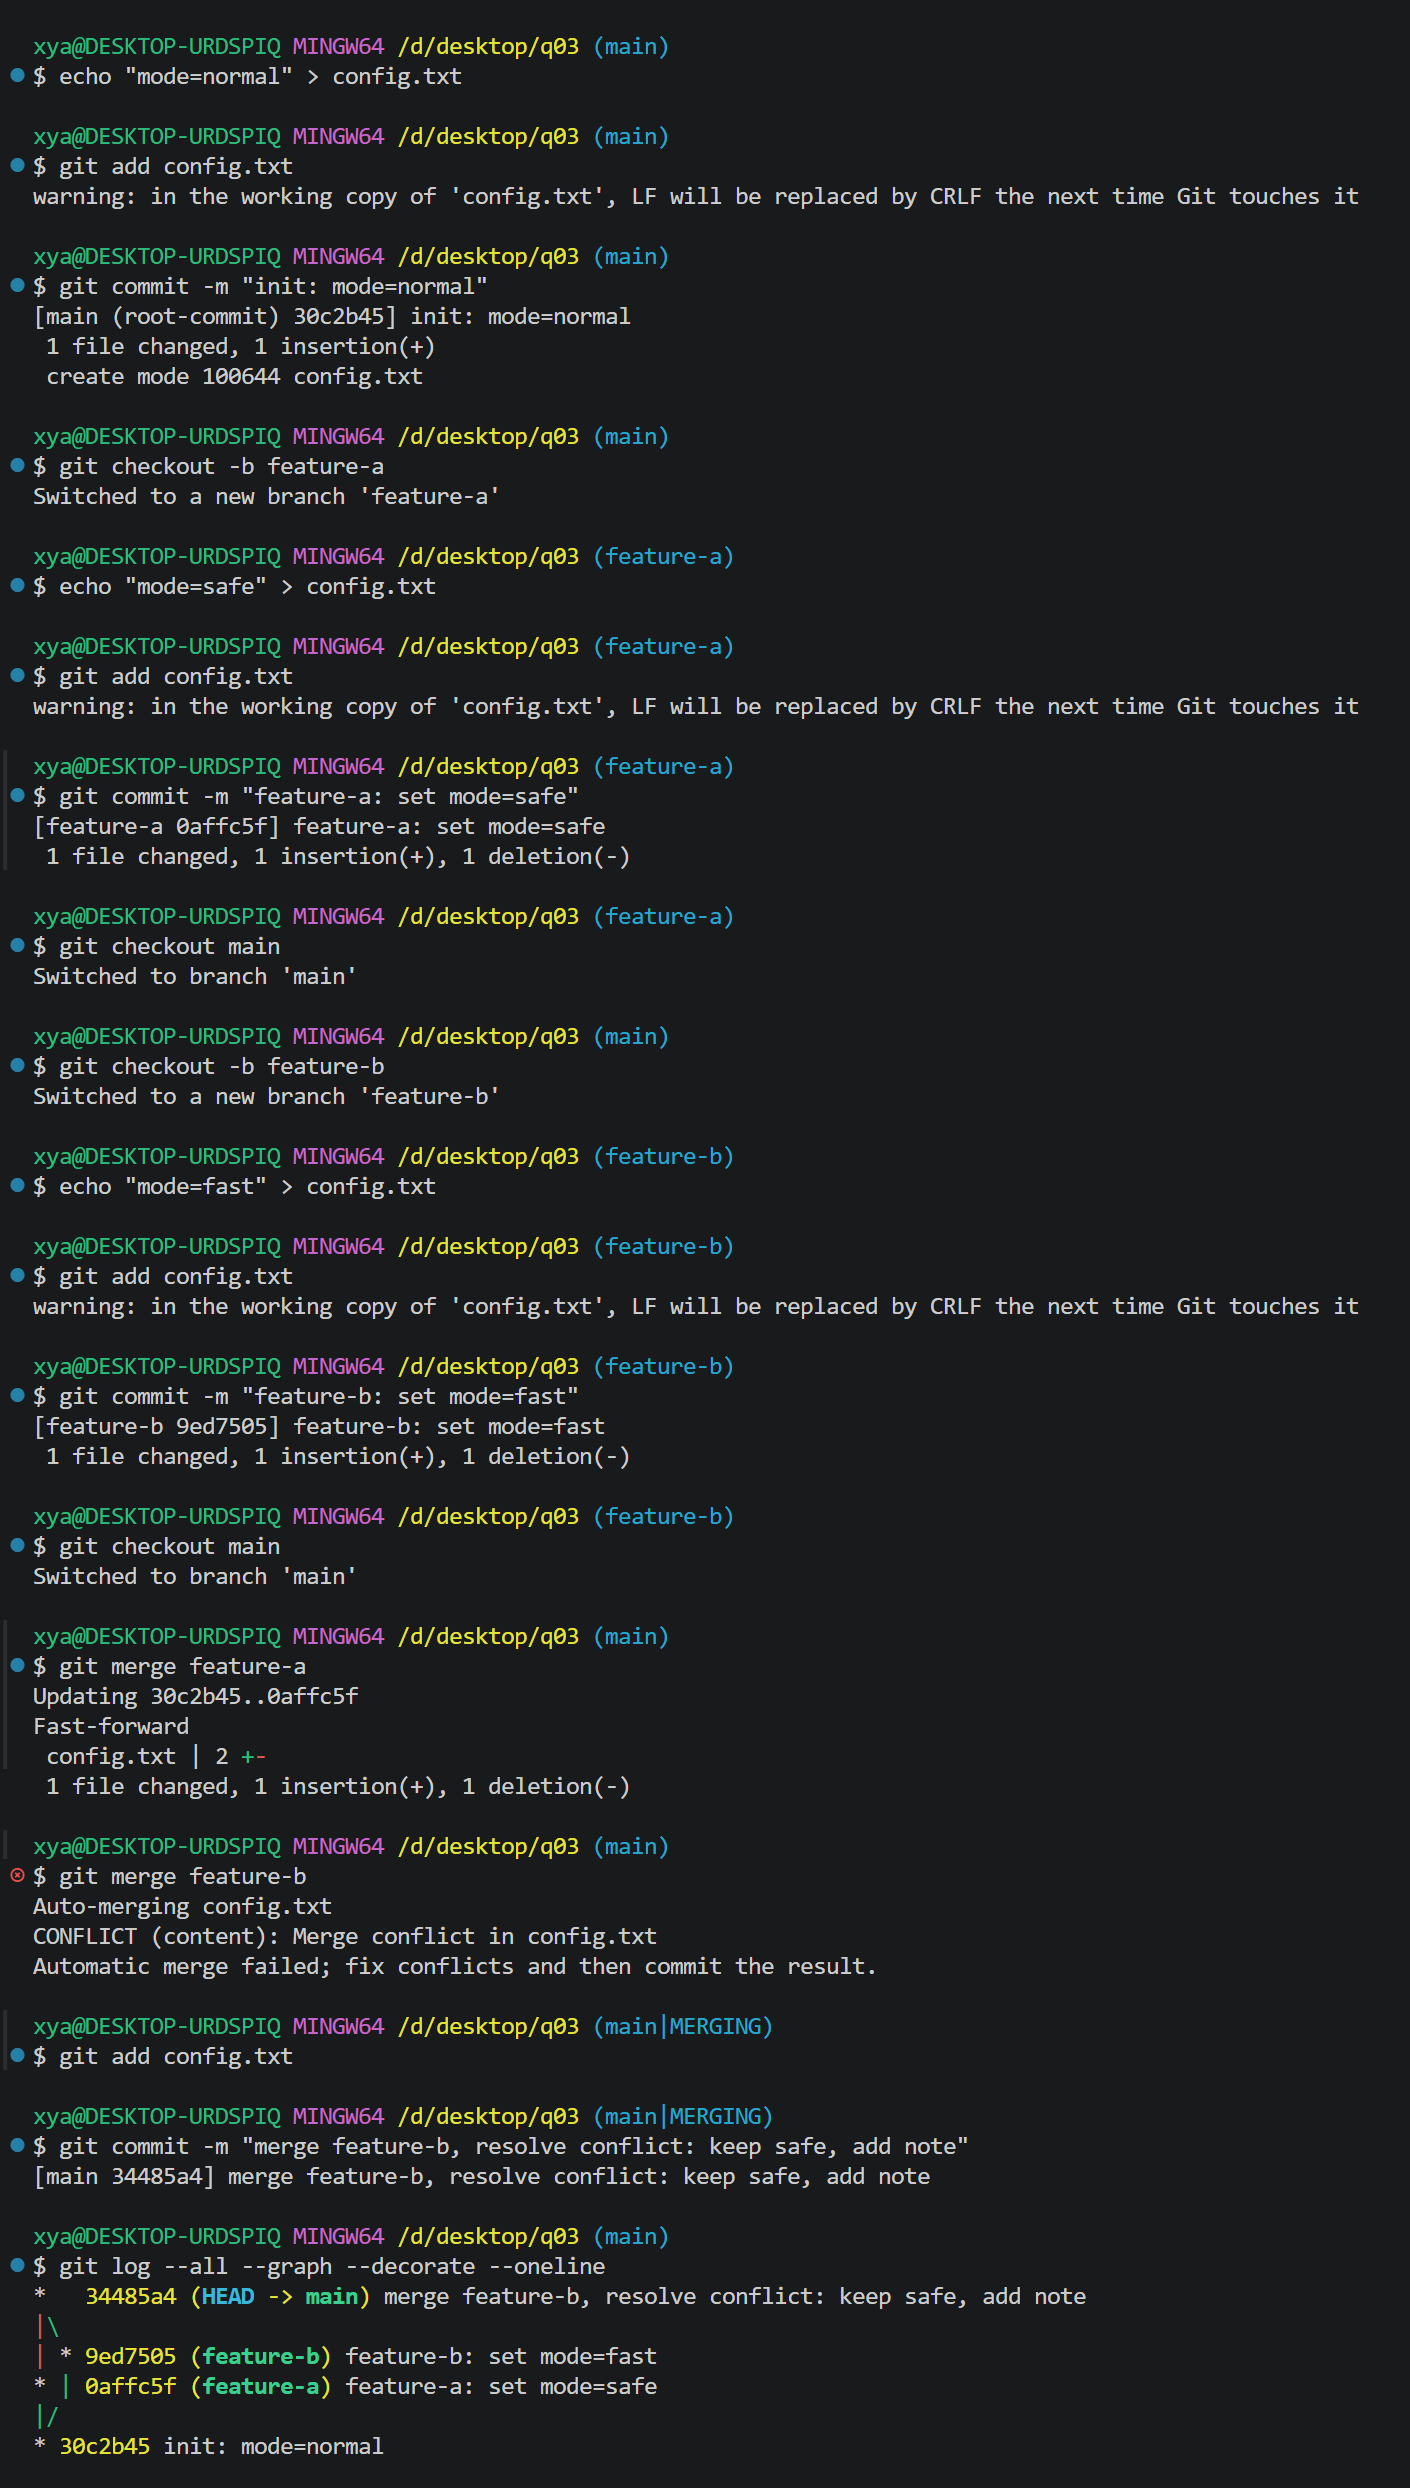
\includegraphics[height=0.96\textheight]{实验过程.png}
  \caption{q03 分支创建、合并冲突与解决的完整过程（终端截图）}
  \label{fig:q03-proc}
\end{figure}

% ================= q04 =================
\subsection{q04 · 修复并构建一页技术说明（LaTeX 文档编辑）}

\begin{taskbox}[题目要求]
将给定模板保存为 q04/report.tex，补全内容并从命令行构建 PDF：
\begin{itemize}[nosep]
  \item 加入一个带编号和 label 的公式，并在正文中使用 ref 或 eqref 引用；
  \item 加入一个 2 行 2 列表格，设置 caption 和 label，并在正文中引用该表；
  \item 使用 \texttt{latexmk -pdf -halt-on-error} 或 tectonic 生成 report.pdf；
  \item 确认 PDF 能打开，且交叉引用不显示“??”。
\end{itemize}
\end{taskbox}

\textbf{实现内容：} 在 \texttt{equation} 环境中加入质能方程，并用
\texttt{\textbackslash eqref} 引用公式编号；随后加入 2 行 2 列表格，并在正文中
引用表格。补全后的源文件见代码~\ref{lst:q04-tex}，构建命令见
代码~\ref{lst:q04-build}。

\lstinputlisting[caption={report.tex：补全后的技术说明},label={lst:q04-tex},language={[LaTeX]TeX}]{课上/q04/report.tex}

\begin{lstlisting}[language=shell,caption={q04 构建命令（TeX Live 2025）},label={lst:q04-build}]
latexmk -pdf -halt-on-error report.tex
\end{lstlisting}

\textbf{编译检查：}
\begin{itemize}[nosep]
  \item \texttt{label} 分别放在公式环境内和表格 \texttt{caption} 之后；
  \item 使用 latexmk 自动完成多轮编译，避免交叉引用显示为“??”。
\end{itemize}

\textbf{结果：} report.pdf 可正常打开，公式和表格的编号、正文引用均正常，
未出现“??”（图~\ref{fig:q04-pdf}）。

\begin{figure}[htbp]
  \centering
  
\includegraphics[page=1,trim=3cm 12.5cm 3cm 4.5cm,clip,width=0.72\textwidth]{课上/q04/report.pdf}
  \caption{q04 构建产物 report.pdf 的主要内容}
  \label{fig:q04-pdf}
\end{figure}

\section{课后练习}

\paragraph{参考资料记录}
\href{https://missing-semester-cn.github.io/2026/course-shell/}{Missing Semester：Shell 入门}、
\href{https://missing-semester-cn.github.io/2020/shell-tools/}{Missing Semester：Shell 工具和脚本}、
\href{https://missing-semester-cn.github.io/2026/version-control/}{Missing Semester：Version Control and Git}、
\href{https://oi-wiki.org/tools/latex/}{OI Wiki：LaTeX 入门}。

\subsection{Shell 练习}

\begin{enumerate}[leftmargin=2.8em,itemsep=0.25em,topsep=0.4em]
  \item \texttt{pwd}：查看当前工作目录，输出绝对路径。
  \item \texttt{ls -lah}：以易读格式列出普通文件、隐藏文件和文件大小。
  \item \texttt{\detokenize{mkdir -p lab/{src,logs,backup}}}：一次创建多层练习目录。
  \item \texttt{\detokenize{printf "alpha\nbeta\n" > data.txt}}：生成两行文本，并用重定向写入文件。
  \item \texttt{\detokenize{cp --parents src/data.txt backup/}}：复制文件并保留相对目录结构。
  \item \texttt{\detokenize{mv data.txt src/input.txt}}：移动文件并同时完成重命名。
  \item \texttt{\detokenize{find lab -type f -name "*.txt"}}：递归查找所有 txt 文件。
  \item \texttt{\detokenize{chmod 640 src/input.txt}}：设置所有者可读写、同组只读的权限。
  \item \texttt{\detokenize{wc -l -w -c src/input.txt}}：同时统计行数、单词数和字节数。
  \item \texttt{\detokenize{grep -nE "alpha|beta" src/input.txt}}：使用扩展正则查找并显示行号。
  \item \texttt{\detokenize{sort names.txt | uniq -c | sort -nr}}：统计重复项并按次数降序排列。
  \item \texttt{\detokenize{cut -d',' -f1,3 scores.csv}}：按逗号分隔提取 CSV 的第 1、3 列。
  \item \texttt{\detokenize{awk -F',' 'NR>1 {sum+=$2} END {print sum}' scores.csv}}：跳过表头并计算第二列总和。
  \item \texttt{\detokenize{sed -E 's/[0-9]+/NUM/g' mixed.txt}}：用正则批量替换文本中的数字。
  \item \texttt{\detokenize{tail -n 20 app.log | head -n 5}}：从日志末尾 20 行中取前 5 行。
  \item \texttt{\detokenize{for f in *.txt; do echo "$f"; done}}：用循环逐个处理匹配到的文件。
  \item \texttt{\detokenize{latest=$(ls -t *.log | head -n 1)}}：使用命令替换取得最新日志文件名。
  \item \texttt{\detokenize{bash script.sh >stdout.log 2>stderr.log}}：分别保存标准输出和标准错误。
  \item \texttt{\detokenize{echo $?}}：检查上一条命令的退出状态，0 表示执行成功。
  \item \texttt{\detokenize{du -ah lab | sort -h}}：统计目录占用空间并按大小排序。
\end{enumerate}

\textbf{练习与结果：} 通过 Shell 中
\texttt{grep}、\texttt{sed}、\texttt{tr}、\texttt{sort}、\texttt{uniq}、
\texttt{awk} 等命令完成检索、状态替换和词频统计，最终得到 8 行、24 个单词，
其中 Git、Shell 和 LaTeX 分别出现 4、3、2 次，相关命令及输出见图~\ref{fig:after-shell}。

\begin{figure}[p]
  \centering
  \resizebox{!}{0.88\textheight}{%
    \vbox{\offinterlineskip
      \hbox{
\includegraphics{课后/shell-notes/1.png}}%
      \hbox{
\includegraphics{课后/shell-notes/2.png}}%
    }%
  }
  \caption{Shell 学习笔记处理与统计过程}
  \label{fig:after-shell}
\end{figure}

\subsection{Git 练习}

\begin{enumerate}[leftmargin=2.8em,itemsep=0.25em,topsep=0.4em]
  \item \texttt{\detokenize{git init git-practice}}：创建独立练习仓库。
  \item \texttt{\detokenize{git status --short}}：用简洁格式查看工作区与暂存区状态。
  \item \texttt{\detokenize{git add README.md}}：把指定文件加入暂存区。
  \item \texttt{\detokenize{git diff}}：查看尚未暂存的修改。
  \item \texttt{\detokenize{git diff --staged}}：查看即将进入下一次提交的修改。
  \item \texttt{\detokenize{git add -p}}：按修改块交互式暂存，拆分不同目的的改动。
  \item \texttt{\detokenize{git commit -m "Add initial notes"}}：创建一次内容集中的提交。
  \item \texttt{\detokenize{git log --all --graph --decorate --oneline}}：以图形方式查看提交 DAG 和分支指针。
  \item \texttt{\detokenize{git switch -c experiment}}：创建并切换到实验分支。
  \item \texttt{\detokenize{git merge --no-ff experiment}}：保留一次明确的合并提交。
  \item \texttt{\detokenize{git stash push -m "unfinished notes"}}：临时保存未完成的修改。
  \item \texttt{\detokenize{git stash list}}：查看暂存的工作现场。
  \item \texttt{\detokenize{git stash pop}}：恢复最近一次 stash 并从列表中移除。
  \item \texttt{\detokenize{git restore README.md}}：丢弃指定文件尚未暂存的修改。
  \item \texttt{\detokenize{git restore --staged README.md}}：把文件移出暂存区但保留工作区修改。
  \item \texttt{\detokenize{git commit --amend}}：补充遗漏内容或修改最近一次提交说明。
  \item \texttt{\detokenize{git rebase -i HEAD~3}}：交互式整理最近三次本地提交。
  \item \texttt{\detokenize{git blame README.md}}：查看每一行最后由哪次提交修改。
  \item \texttt{\detokenize{git show HEAD:README.md}}：直接查看 HEAD 快照中的文件内容。
  \item \texttt{\detokenize{git cat-file -p HEAD^{tree}}}：查看提交指向的树对象，联系 Git 的对象模型。
\end{enumerate}

\textbf{练习与结果：} 在独立仓库中完成分块暂存、三次提交、stash 恢复、
\texttt{restore} 撤销、\texttt{amend} 补充提交和 \texttt{v1.0} 标签，并用
\texttt{log}、\texttt{show}、\texttt{blame} 与 \texttt{cat-file} 验证了最终历史和文件内容，
相关操作记录见图~\ref{fig:after-git-1} 和图~\ref{fig:after-git-2}。

\begin{figure}[p]
  \centering
  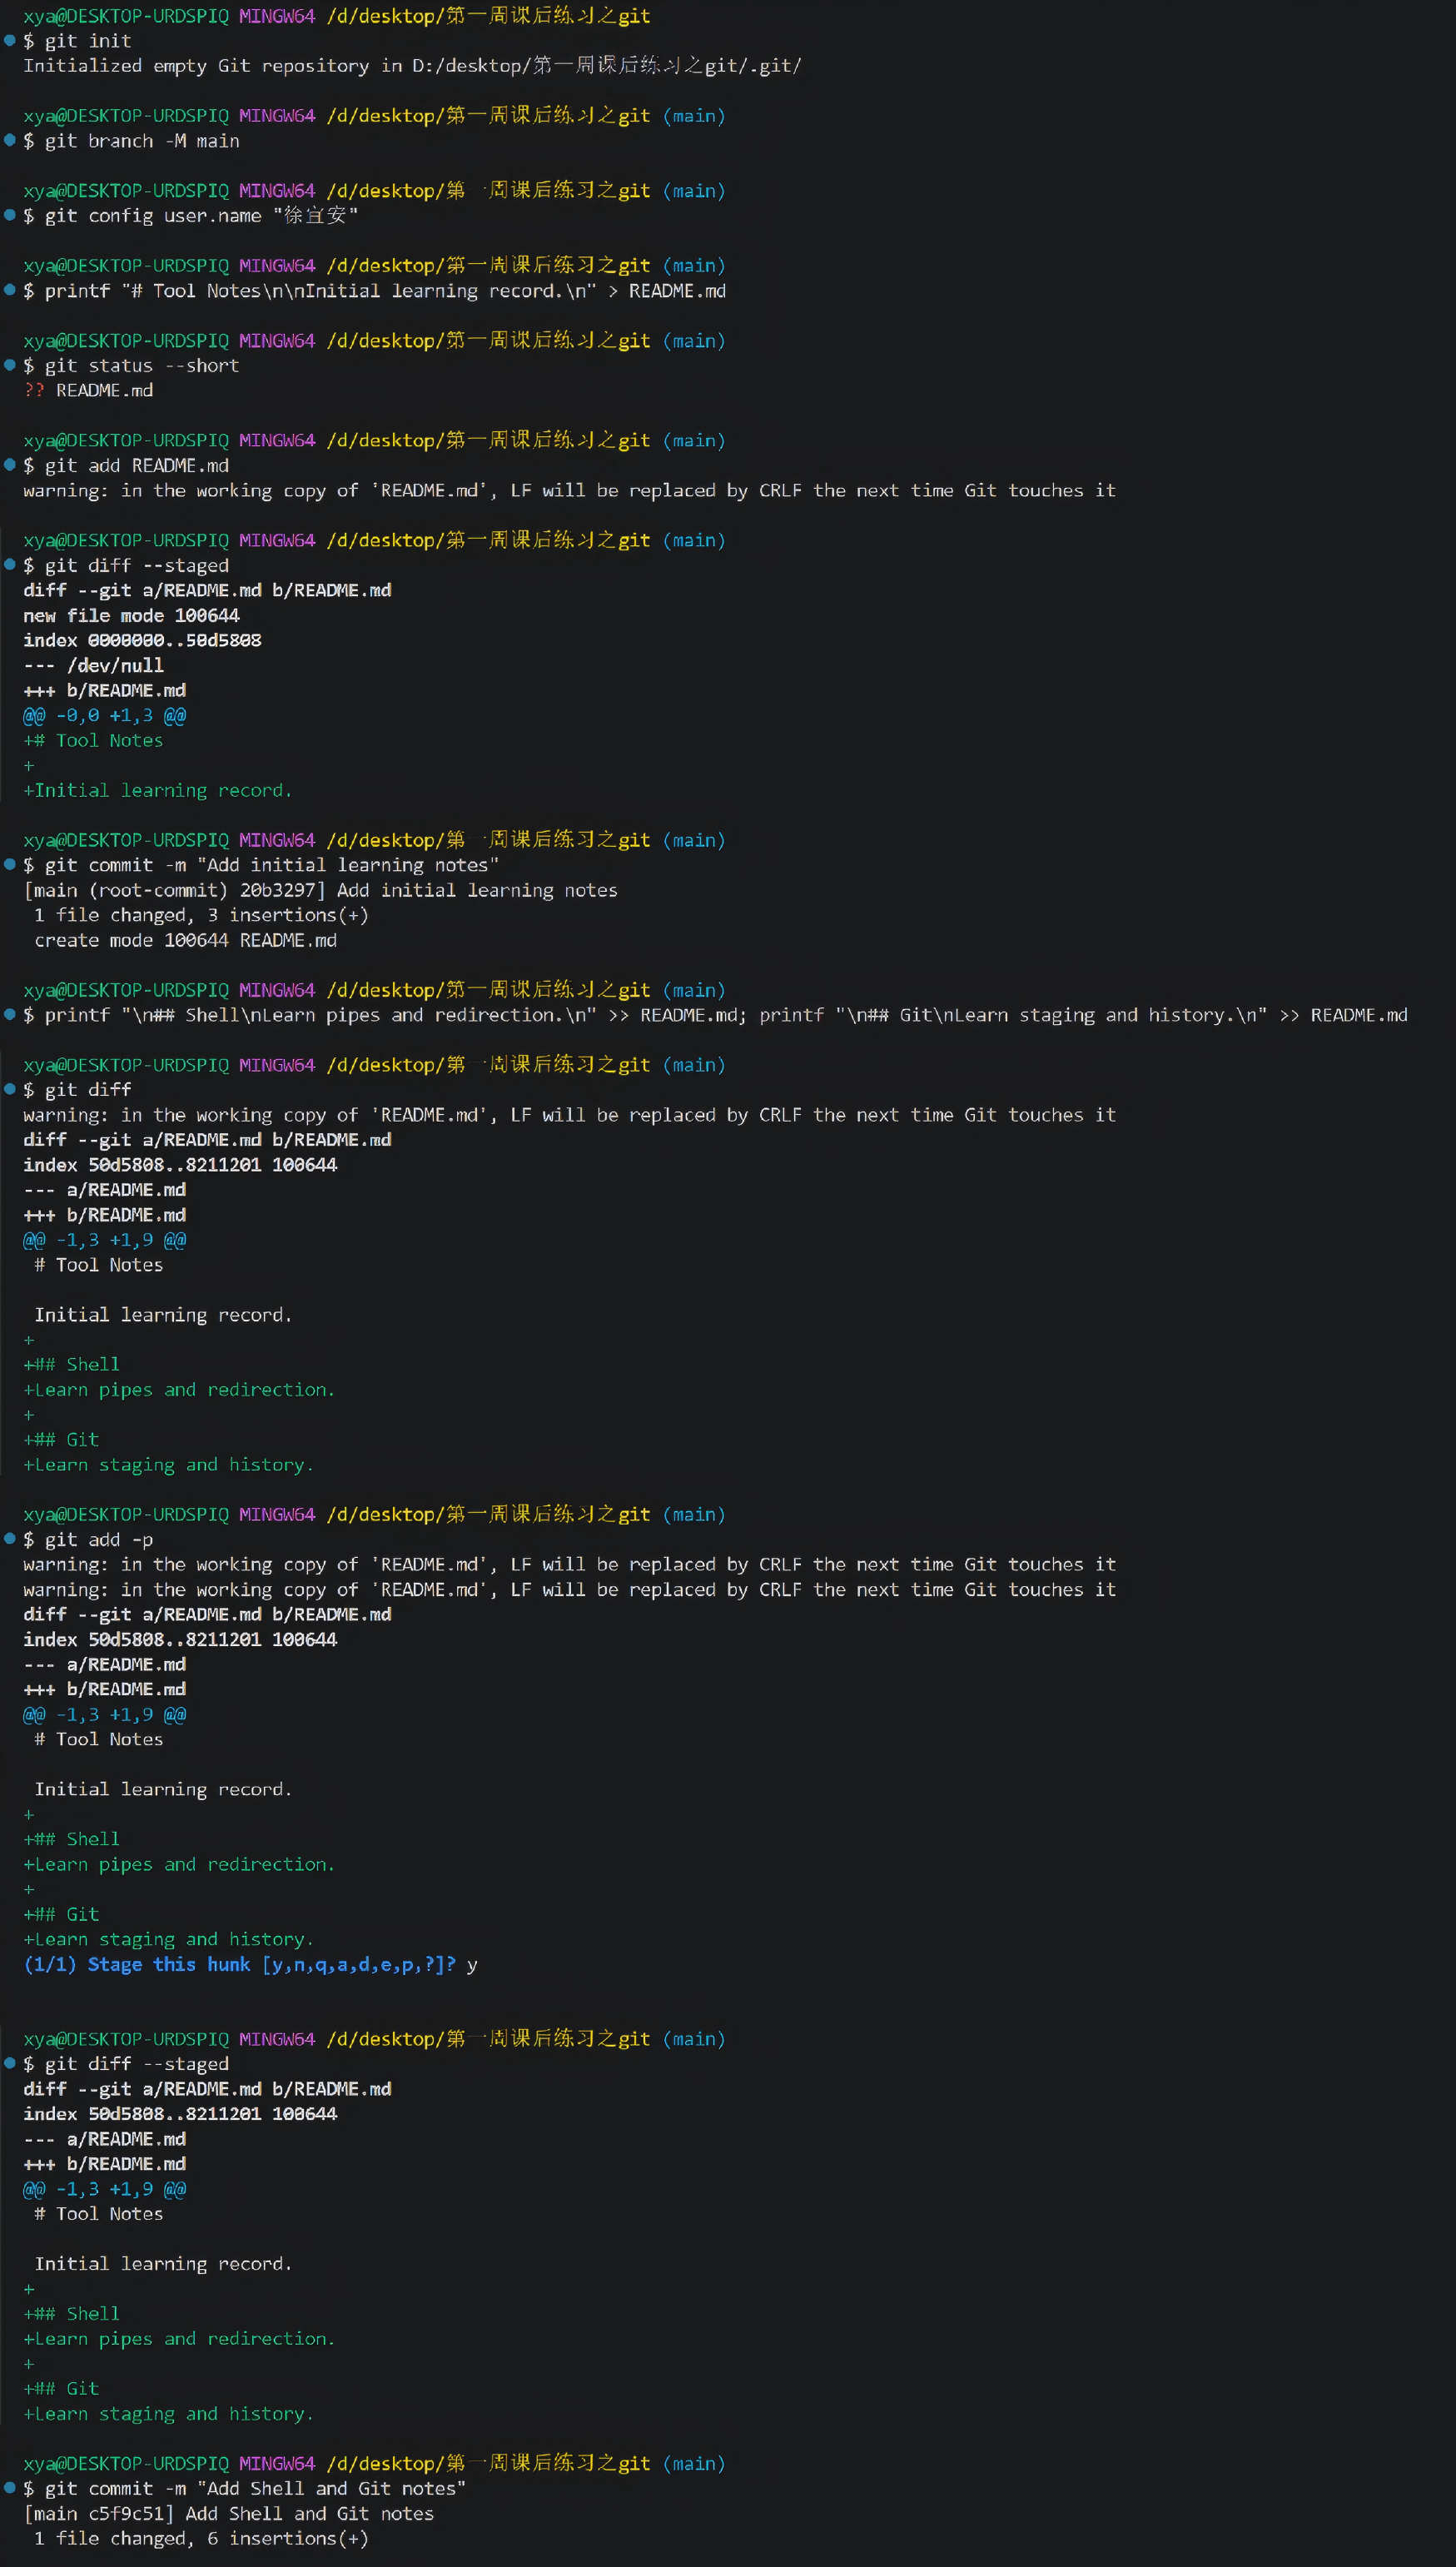
\includegraphics[height=0.96\textheight]{课后/git-notes/1.png}
  \caption{Git 练习：初始化、差异查看、分块暂存与提交}
  \label{fig:after-git-1}
\end{figure}

\begin{figure}[p]
  \centering
  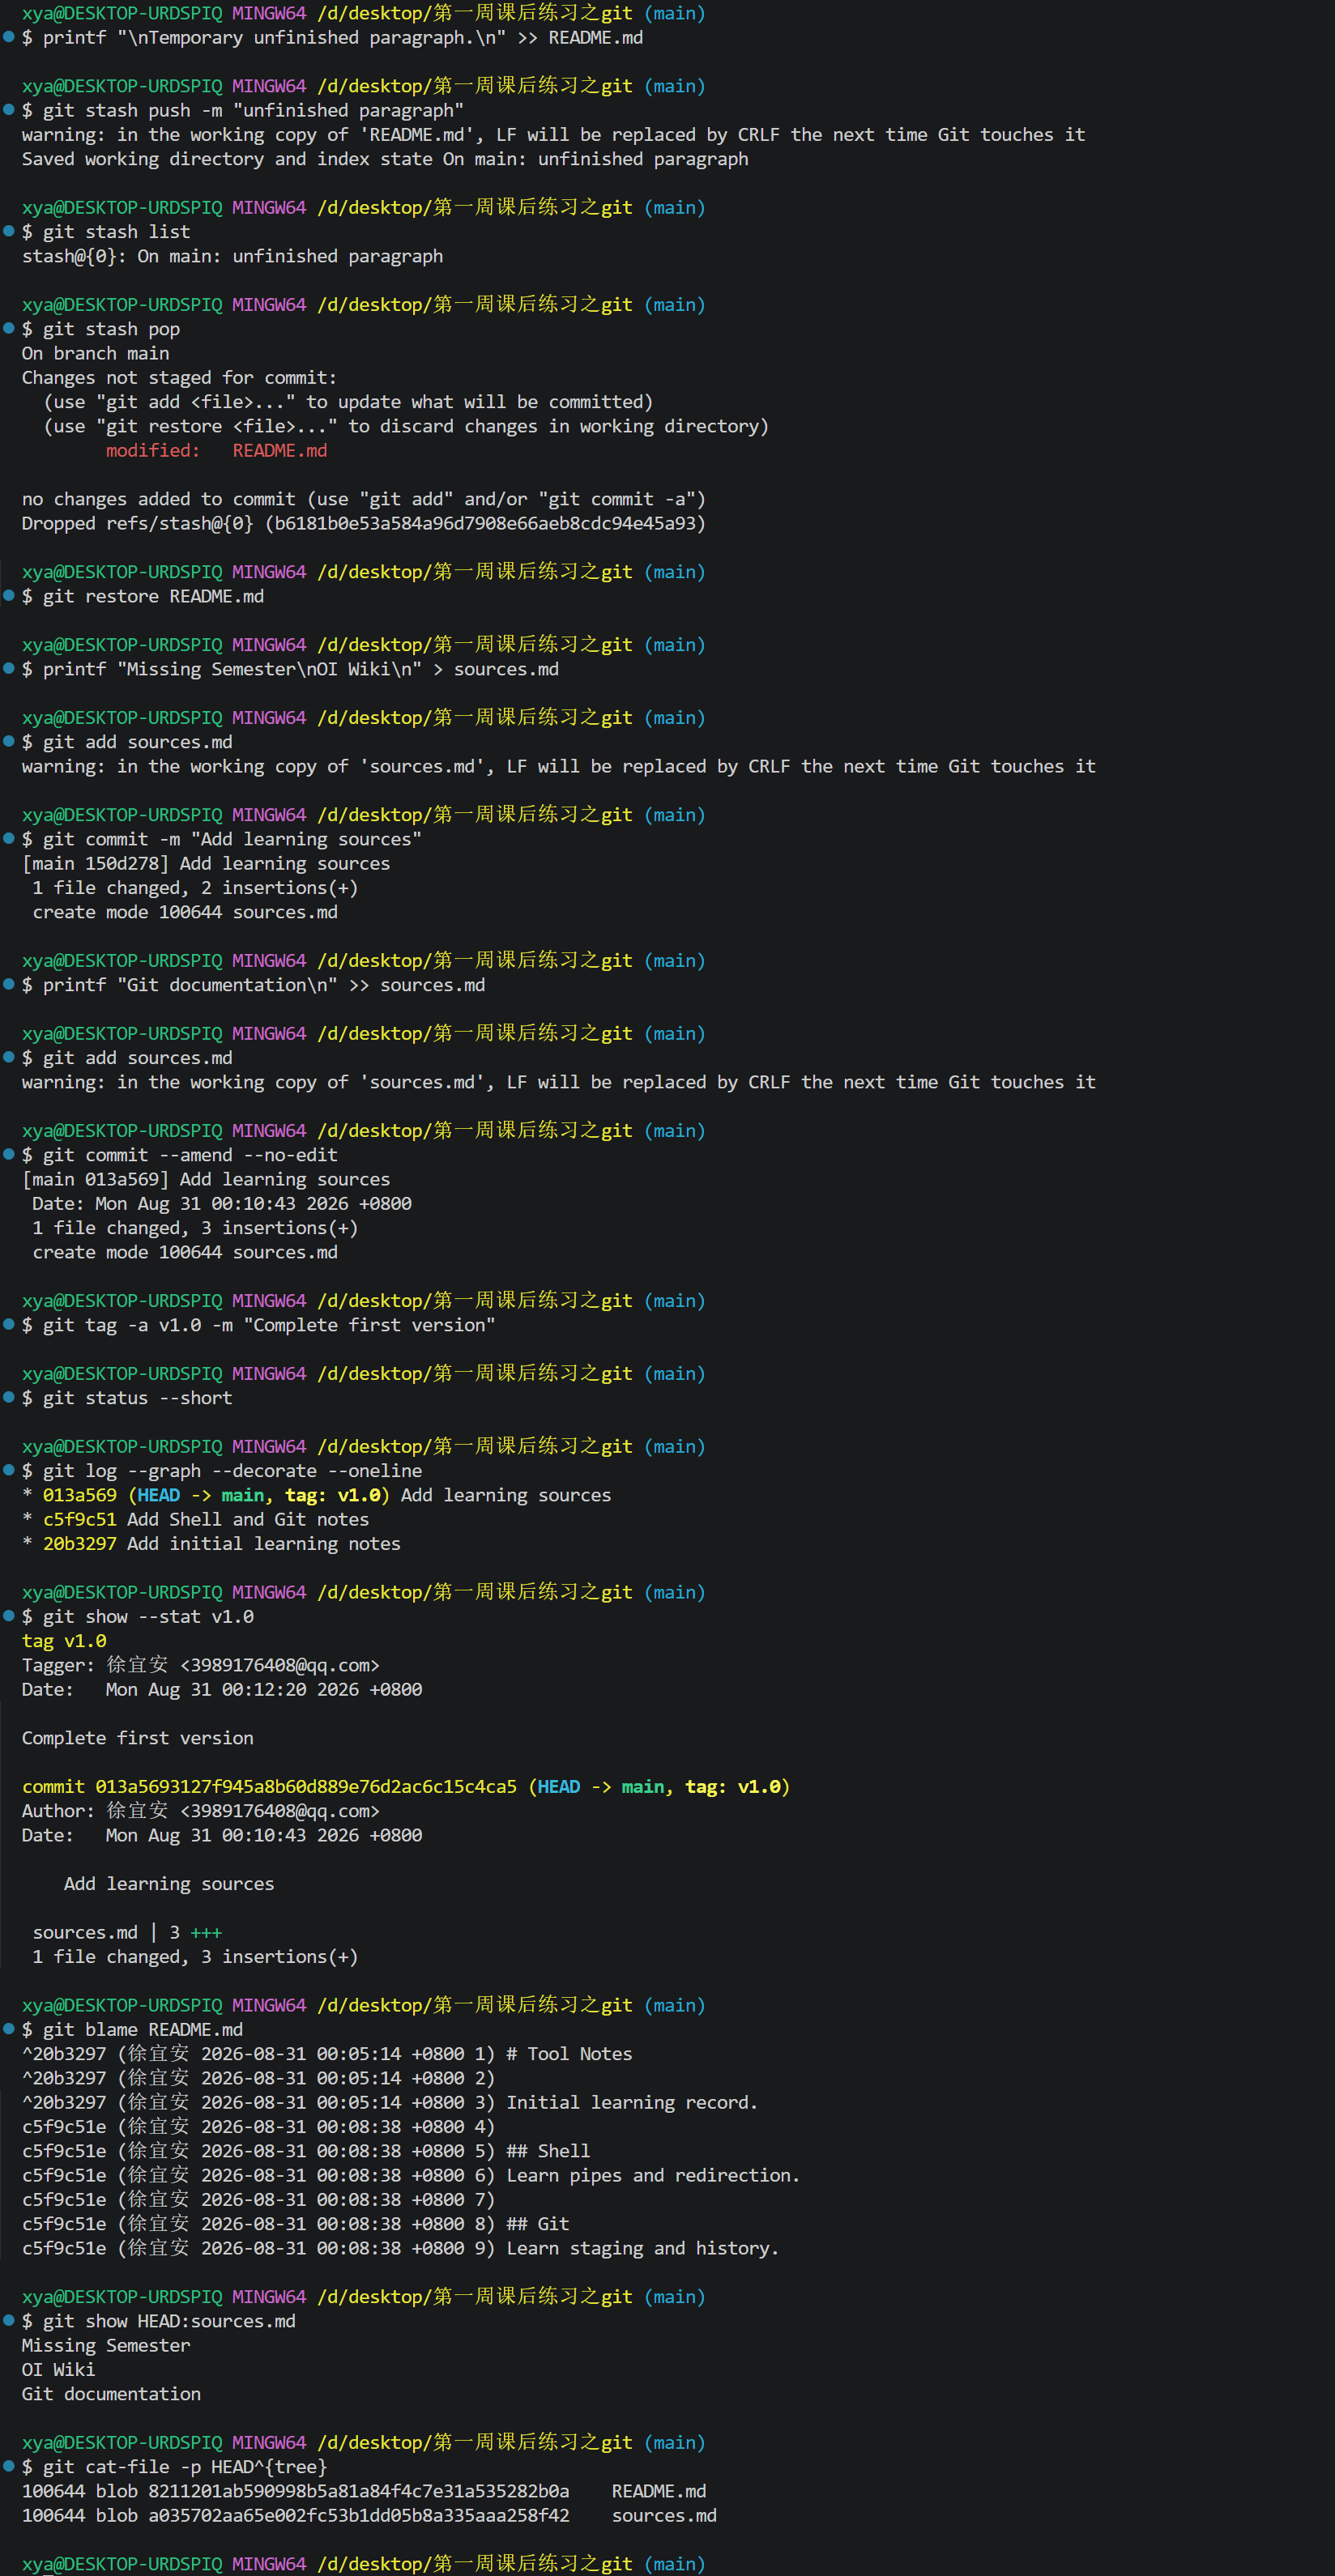
\includegraphics[height=0.96\textheight]{课后/git-notes/2.png}
  \caption{Git 练习：stash、撤销、amend、标签与历史验证}
  \label{fig:after-git-2}
\end{figure}

\subsection{LaTeX 练习}

\begin{enumerate}[leftmargin=2.8em,itemsep=0.25em,topsep=0.4em]
  \item 用 \texttt{ctexart} 写中文文档，使中文能够正常排版。
  \item 设置 \texttt{title}、\texttt{author}、\texttt{date}，用 \texttt{maketitle} 生成标题。
  \item 用 \texttt{section}、\texttt{subsection} 建立两级文档结构。
  \item 用 \texttt{tableofcontents} 生成目录，需要通过多轮编译更新页码。
  \item 用 \texttt{itemize} 排版无序列表，调整列表间距。
  \item 用 \texttt{enumerate} 排版自动编号列表。
  \item 用 \texttt{\detokenize{$E=mc^2$}} 插入行内公式。
  \item 用 \texttt{equation}、\texttt{label} 和 \texttt{eqref} 创建并引用带编号公式。
  \item 用 \texttt{align} 对齐多行推导中的等号。
  \item 用 \texttt{pmatrix} 排版矩阵，并检查括号和列对齐。
  \item 用 \texttt{cases} 排版分段函数。
  \item 用 \texttt{tabular} 创建表格，设置列对齐方式。
  \item 引入 \texttt{booktabs}，用 \texttt{toprule}、\texttt{midrule}、\texttt{bottomrule} 改进表格线条。
  \item 用 \texttt{caption}、\texttt{label}、\texttt{ref} 完成表格编号与正文引用。
  \item 引入 \texttt{graphicx}，用 \texttt{includegraphics} 插入图片并按正文宽度缩放。
  \item 引入 \texttt{hyperref}，用 \texttt{href} 添加可点击的网页链接。
  \item 用 BibTeX 建立 \texttt{.bib} 文件，通过 \texttt{cite} 插入并生成参考文献。
\end{enumerate}

\textbf{练习与结果：} 使用 LaTeX 在一页中展示列表、公式、矩阵、分段函数、
三线表、图片、超链接和 BibTeX 文献引用，最终 PDF 编号与交叉引用均正常，
编译结果见图~\ref{fig:after-latex}。
完整代码见 \texttt{课后/latex-planner/planner.tex}，核心部分如下。

\begin{lstlisting}[
  language={[LaTeX]TeX},
  basicstyle=\scriptsize\ttfamily,
  numbers=none,
  caption={planner.tex 核心代码（排版参数略）},
  label={lst:after-latex}
]
\documentclass[10pt,a4paper]{ctexart}
\usepackage{amsmath,booktabs,graphicx,caption,hyperref}
\begin{document}
\section{文档结构}
\begin{itemize}
  \item Shell 命令 \item Git 版本控制 \item LaTeX 排版
\end{itemize}
行内公式 $E=mc^2$。
\begin{equation} S=0.4A+0.6B \label{eq:score} \end{equation}
公式~\eqref{eq:score}表示加权成绩。
\begin{align} x+y&=10, & x-y&=2. \end{align}
\[
A=\begin{pmatrix}1&2\\3&4\end{pmatrix},\qquad
f(x)=\begin{cases}x,&x\ge0,\\-x,&x<0.\end{cases}
\]
\captionof{table}{学习安排}\label{tab:plan}
\begin{tabular}{ccc}
\toprule 工具&时间&状态\\ \midrule
Shell&2 h&完成\\ Git&3 h&完成\\ LaTeX&2 h&进行中\\
\bottomrule
\end{tabular}
\includegraphics[width=.3\textwidth]{example-image-a}
\href{https://missing-semester-cn.github.io/}{Missing Semester}
正文引用参考资料~\cite{missingsemester}。
\bibliographystyle{unsrt}
\bibliography{references}
\end{document}
\end{lstlisting}

\begin{figure}[htbp]
  \centering
  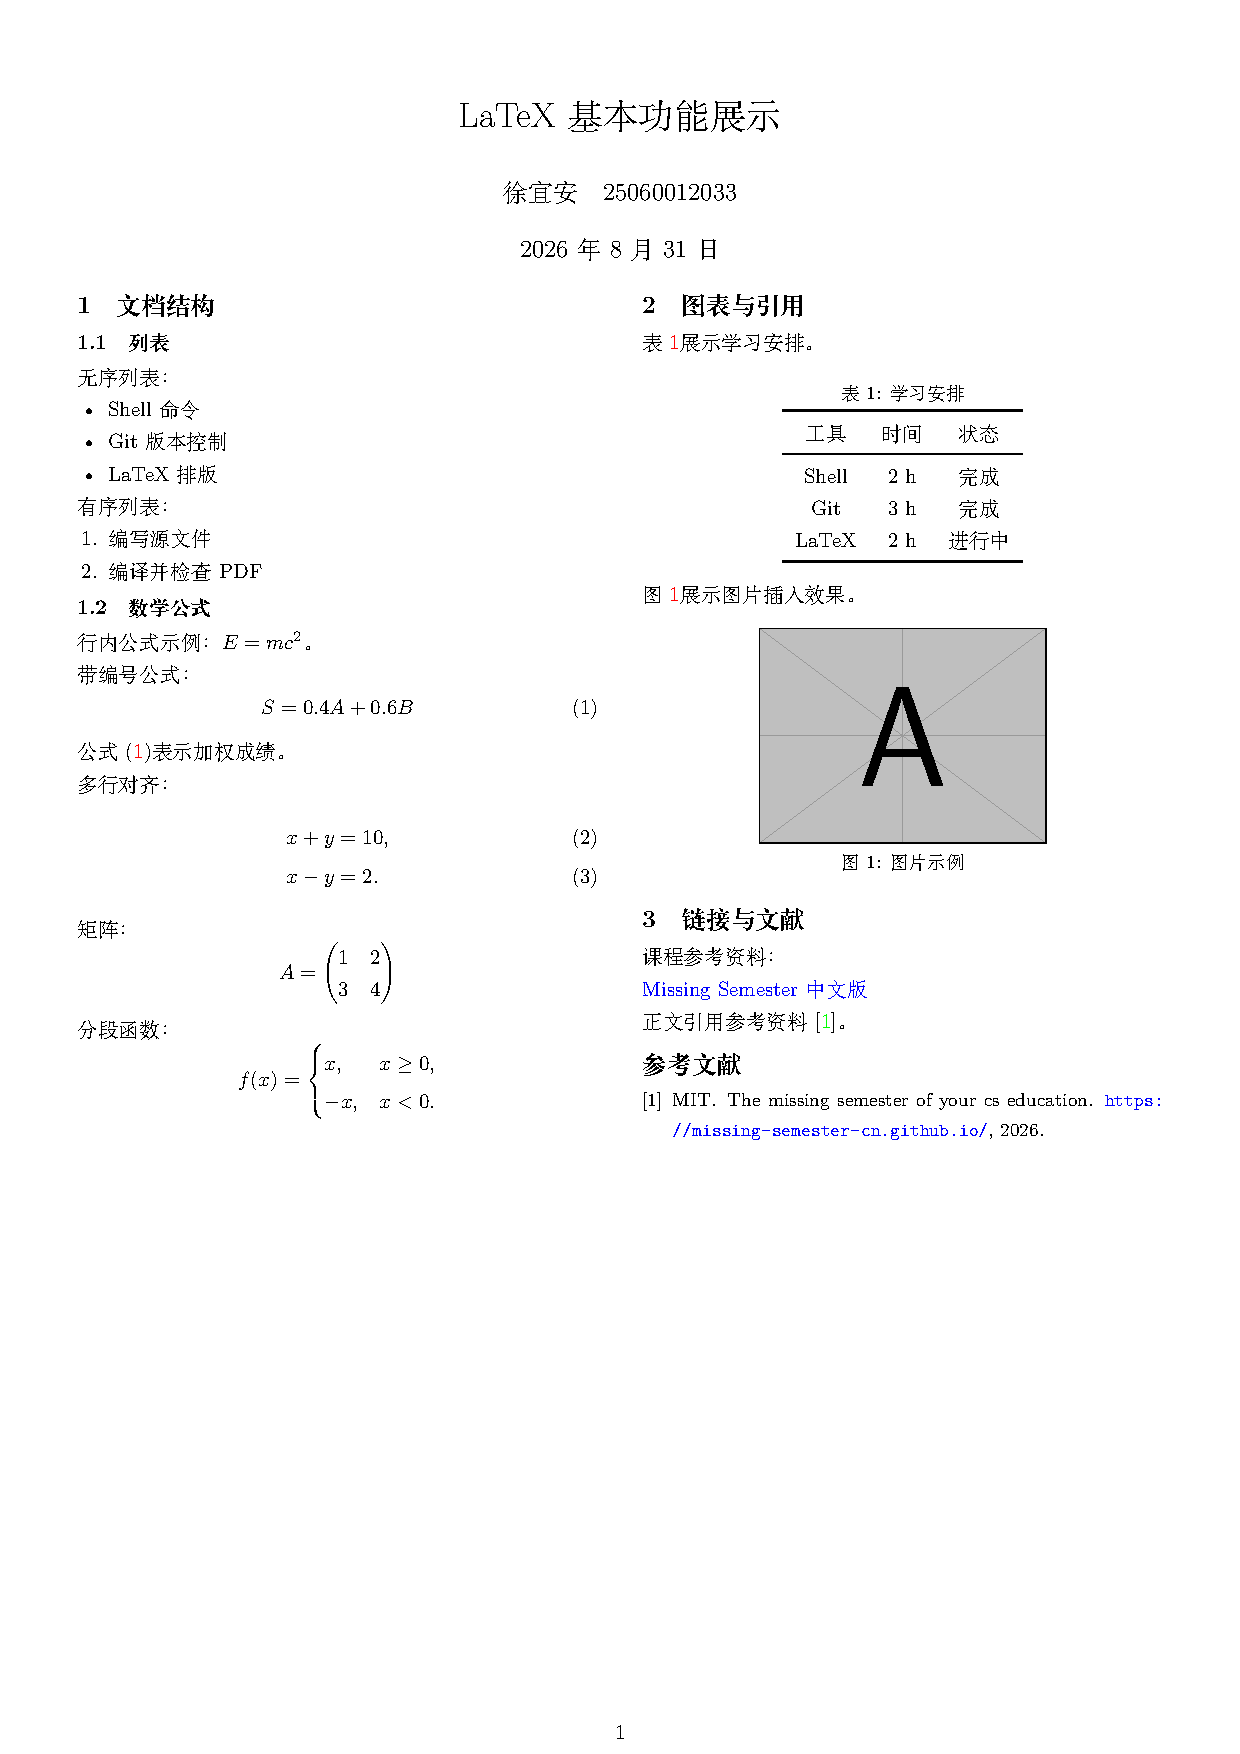
\includegraphics[page=1,trim=0 8cm 0 0,clip,width=0.68\textwidth]{课后/latex-planner/planner.pdf}
  \caption{LaTeX 基本功能展示的编译结果}
  \label{fig:after-latex}
\end{figure}

\section{解题感悟}

先记录下我这周学会了什么吧。之前大概只会一些基本的文件操作的命令，一直没搞明白shell、bash、Terminal这几个东西的关系，感觉都差不多，
现在知道Terminal是输入文字用的交互地方，shell解释命令沟通操作系统，bash是其中一种shell，
还有关于脚本也有所了解了（之前好像还是挺怕这种东西的）。关于git我之前会在本地用些最简单的add、commit等命令，这次熟练了推送远程仓库
（还知道怎么快速使用Vscode插件中的gui界面了，git其它gui工具反而不喜欢不想用），以及关于分支之前没有好好学，这次收获了合并分支解决冲突。
关于Latex之前有通识课结课论文用过，但是具体语法没那么熟，更习惯用语法更简单的md来写然后让ai给我转成Latex编译，这次更加熟悉了吧，
还对不同配方更有了解。

我有在思考ai时代下我应该优先掌握什么（有的指令好难记啊我感觉不常用根本记不住）。首先肯定是得学过、跟着理解过这些工具，这些是基础，
之后如果要用可以知道是什么有什么用，不常用的命令或者语法记不住可以问ai或者查文档教程。其次是一些程序员必备的技能了，
比如基本的shell命令、git命令，这些肯定要牢记。现在我可能awk、sed这种复杂命令还不太熟，Latex让我直接写估计也只能写个结构，
但是感觉更值得学的还是git，把分支学明白。

最近越来越体会到学计算机需要接触自己陌生的新事物，学技术，也希望自己能从这四周的课开始好好实践吧。

第一周课上实验、课后练习及实验报告均已提交至 Git 仓库，相关提交记录见图~\ref{fig:commit-record}。

\begin{center}
  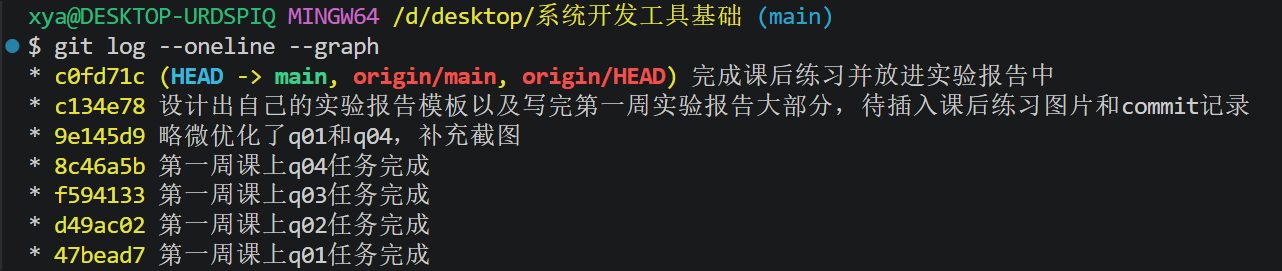
\includegraphics[width=\textwidth]{commit记录.png}
  \captionof{figure}{第一周实验及报告的 Git 提交记录}
  \label{fig:commit-record}
\end{center}

\end{document}
